\section{Robotic Architecture Design} \label{sec:architecture}
The robot's software has been constructed from existing and proven components as much as possible. The lowest level of the architecture is the Melodic Morenia distribution of ROS. SkiROS2 \cite{skiros2} manages the robot's skills and handles task planning. MoveIt \cite{moveit} is responsible for controlling the motion of the manipulator arm. The Navigation Stack \cite{navigation_stack} handles simultaneous localization and mapping (SLAM) and wheel control. Figure \ref{fig:paintbot_arch} shows a high-level description of these components and their relations.

\begin{figure}
    \centering
    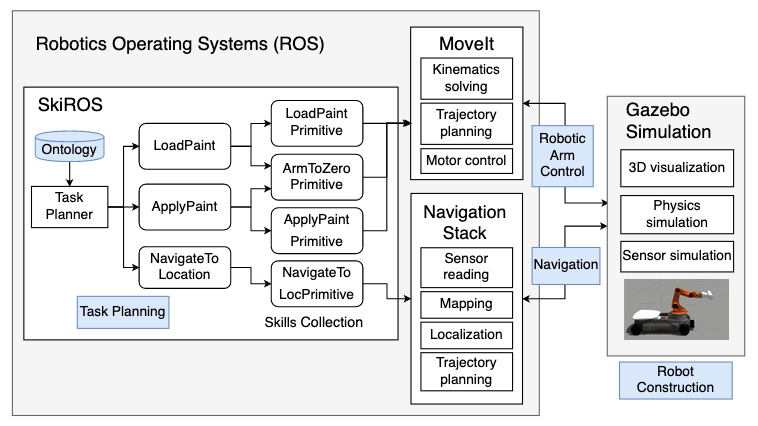
\includegraphics[width=1.0\linewidth]{images/architecture.png}
    \caption{A high-level diagram of the robot's software components and simulation environment. The arrows indicate the direction of communication and the rounded boxes indicate skills implemented for this research and are not native components of SkiROS.}
    \label{fig:paintbot_arch}
\end{figure}

\subsection{Robot Construction}
The hardware of the robot is based on the KUKA youBot, a robot designed for education and industrial research. It comes equipped with a manipulator arm with $5$ degrees of freedom, four omni wheels that enable holonomic motion, and a front-mounted laser rangefinder. The gripper at the end of the manipulator arm was replaced with a paint roller to enable the robot to carry out the painting task. Fully extended, the arm reaches \SI{0.655}{\meter} vertically or \SI{0.5405}{\meter} horizontally. The holonomic motion allows the robot to make more accurate adjustments to its position and to better align itself with its target. The laser has a range of \SI{10}{\meter}, a \ang{180} arc, and \SI{0.01}{\meter} resolution.

\subsection{Ontology} \label{sec:ontology}
A small ontology, given the working title of the {\tt paintbot} ontology for the purposes of this paper, was created to represent the entities relevant to the robot during its painting tasks. This ontology is encoded in Web Ontology Language (OWL) and is used during planning. The {\tt paintbot} ontology includes the CORA \cite{ieee2015cora}, SUMO \cite{sumo}, and SkiROS ontologies and makes use of several concepts from them.

The {\tt paintbot} ontology contains the following concepts (see Figure~\ref{fig:paintbot_ontology} for a visual representation):
\begin{itemize}
    \item The Paint class represents fluid paint.
    \item The PaintTray class represents the trays that hold paint for use with paint rollers.
    \item The WallSection class represents a short section of wall that can be painted in the single execution of a skill. In this research, a WallSection is no wider than one standard paint roller (see section \ref{sec:implementation}).
    \item The hasColor object property relates any object to a Paint. This represents an object being coated in paint and is most commonly used with WallSections and the robot arm.
    \item The targetColor object property relates any object to a Paint. This represents the requirement of an object needing to be painted and is currently only used with WallSections.
    \item The Painted data property is a boolean property that denotes if an object is painted (i.e. its hasColor and targetColor relations refer to the same Paint). This was created to aid in skill definition and planning.
\end{itemize}

\begin{figure}
    \centering
    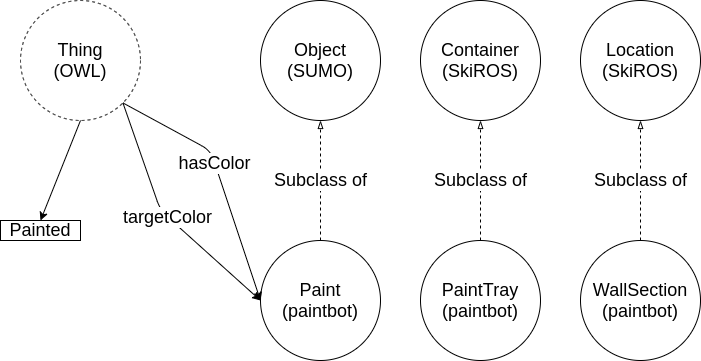
\includegraphics[width=0.95\linewidth]{images/ontology.png}
    \caption{A diagram of the concepts in the {\tt paintbot} ontology. The Thing class comes from OWL, the Object class comes from SUMO, and both the Container and Location classes come from the SkiROS ontology.}
    \label{fig:paintbot_ontology}
\end{figure}

%%%% peggy mark %%%%%
%This ontology, much like the research as a whole, is an initial proof of concept and is intended to be extended as more functionality and flexibility is added to the robot. It is intended that this could form the basis of a larger ontology that standardizes a wide range of construction knowledge for use with robotics.

\subsection{Task Planning} \label{sec:task_planning}
SkiROS2 is the evolution of the original SkiROS system developed by Rovida et al. \cite{rovida2017skiros}. This provides a framework for specifying the robot's skills and supports goal-directed task planning using planning domain definition language (PDDL). SkiROS requires an ontology for the problem domain to be defined in addition to the robot's skills. Once the ontology and skills are properly defined, PDDL goals may be provided to SkiROS to cause it to plan a sequence of tasks for the robot to perform.


A robot skill is a behavior or functionality of a robot. An
example of a robot skill is the capability to move a robot arm to follow a certain trajectory. Skills defined here are classified as either (1) {\it primitive skill}, which is
directly responsible for causing the robot to take action, or (2) {\it compound skill}, which is defined in terms of one or more primitive skills or other compound skills and control how the execution of the subskills proceeds (e.g., sequentially, concurrently, how failures are handled, etc.). Due to the nature of PDDL, SkiROS skill definitions include parameters, conditions, and effects in order to be utilized in planning. The high-level summary of the skills defined here are%\footnote{The full PDDL of the skills, as generated by SkiROS, can be found in Appendix \ref{app:skill_pddl}}:
\begin{itemize}
    \item {\bf NavigateToLocationPrimitive} (primitive skill): This skill coordinates with the Navigation Stack to move the robot to the Destination.
    \begin{itemize}
        \item {\bf Parameters} - Destination
        %\item This skill coordinates with the Navigation Stack to move the robot to the Destination.
    \end{itemize}
    
    \item {\bf NavigateToLocation} (compound skill): This skill invokes NavigateToLocationPrimitive and ensures that the relations governing the robot's position are properly set for the planner.
    \begin{itemize}
        \item {\bf Parameters} - Start, Destination, Robot
        \item {\bf Conditions} - Robot is at Start, Robot is not at Destination
        \item {\bf Effects} - Robot is not at Start, Robot is at Destination
        %\item The skill invokes the NavigateToLocationPrimitive and ensures that the relations governing the robot's position are properly set for the planner.
    \end{itemize}
    
    \item {\bf ArmToZeroPrimitive} (primitive skill): This skill coordinates with MoveIt to move the arm to its {\it zero position}, a default position that does not extend past the edges of the robot's body.
    %\begin{itemize}
        %\item This skill coordinates with MoveIt to move the arm to its {\it zero position}, a default position that does not extend past the edges of the robot's body.
    %\end{itemize}
    \item {\bf LoadPaintPrimitive} (primitive skill): This skill coordinates with MoveIt to generate the arm motion that loads the specified Paint onto the paint roller from a paint tray in front of the robot.
    \begin{itemize}
        \item {\bf Parameters} - Paint, Arm
        %\item This skill coordinates with MoveIt to generate the arm motion that loads the specified Paint onto the paint roller from a paint tray in front of the robot.
    \end{itemize}
    
    \item {\bf ApplyPaintPrimitive} (primitive skill): This skill coordinates with MoveIt to generate the arm motion that paints the specified Wall in front of the robot with the specified Paint.
    \begin{itemize}
        \item {\bf Parameters} - Paint, Wall, Arm
        %\item This skill coordinates with MoveIt to generate the arm motion that paints the specified Wall in front of the robot with the specified Paint.
    \end{itemize}
    
    \item {\bf LoadPaint} (compound skill): This skill sequentially invokes LoadPaintPrimitive and ArmToZeroPrimitive.
    \begin{itemize}
        \item {\bf Parameters} - Paint, Tray, Arm, Robot
        \item {\bf Conditions} - Arm does not have Paint, Tray contains Paint, Robot is at Tray
        \item {\bf Effects} - Arm has Paint
        %\item This skill sequentially invokes the LoadPaintPrimitive and the ArmToZeroPrimitive.
    \end{itemize}
    
    \item {\bf ApplyPaint} (compound skill): This skill sequentially invokes ApplyPaintPrimitive and ArmToZeroPrimitive.
    \begin{itemize}
        \item {\bf Parameters} - Paint, Wall, Arm, Robot
        \item {\bf Conditions} - Wall is not Painted, Wall must be painted with Paint, Arm has Paint, Robot is at Wall
        \item {\bf Effects} - Wall is painted with Paint, Wall is Painted, Arm does not have Paint
        %\item This skill sequentially invokes the ApplyPaintPrimitive and the ArmToZeroPrimitive.
    \end{itemize}
    
    \item {\bf GeneratePaintSubGoalPrimitive} (primitive skill): This skill finds up to $10$ wall sections that have yet to be painted and constructs a PDDL goal for them. Goal is used as an output parameter that contains the constructed PDDL and is utilized by subsequent skills in the plan.
    \begin{itemize}
        \item {\bf Parameters} - Goal
        %\item This skill finds up to $10$ wall sections that have yet to be painted and constructs a PDDL goal for them. Goal is used as an output parameter that contains the constructed PDDL and is utilized by subsequent skills in the plan.
    \end{itemize}
    
    \item {\bf PaintAllWallSections} (compound skil): This skill uses the GeneratePaintSubGoalPrimitive skill to generate a series of tasks that in turn generate painting plans for small groups of wall sections at a time (see section \ref{sec:implementation} for more explanation)
    %\begin{itemize}
        %\item This skill uses the GeneratePaintSubGoalPrimitive skill to generate a series of tasks that in turn generate painting plans for small groups of wall sections at a time (see section \ref{sec:implementation} for more explanation).
    %\end{itemize}
\end{itemize}

Planning in SkiROS is performed by the Temporal Fast Downward (TFD) planner created by Eyerich, Mattm{\"u}ller, and R{\"o}ger \cite{eyerich2009using}. TFD is an extension of the original Fast Downward planner created by Helmert \cite{helmert2006fast}. TFD uses the PDDL derived from the skills to generate a sequence of skills that achieve the given PDDL goal. %A cursory investigation suggests that TFD could be replaced with another algorithm with a reasonable amount of effort for the future work. %, but this option was not pursued during this stage of the research.

\subsection{Robotic Arm Control}
The MoveIt package provides a common and proven framework for the configuration, trajectory planning, and motor control of robotic manipulator arms. During the development of the robot, a large number of errors were encountered while attempting to plan trajectories for the paint loading and application motions. To alleviate this, the default KDL kinematics solver was replaced with the TRAC-IK solver \cite{trac_ik}. MoveIt comes packaged with many trajectory planners, though the default RRTConnect planner \cite{kuffner2000rrt} was used as it proved satisfactory in generating plans for the arm motions required by our current design.

\subsection{Navigation}
SLAM is the problem of finding solutions for autonomous navigation in unknown environments and can be decomposed into the two primary components of its namesake: mapping and localization. 
%%%%%%% peggy %%%%%%%%%
%Mapping is the act of collecting information about the environment and constructing an internal representation of its layout. Maps are commonly concerned with representing navigable terrain, obstacles, and elevation. Localization is the act of estimating where the robot is located inside the map. Landmark identification, odometry, and sensor data, such as that from GPS, are all combined to make this estimation.
The Navigation Stack is a framework that provides both SLAM and motor control functionality. It has three primary subcomponents that need to be configured for the robot: 1) the mapping component, 2) the localization component, and 3) the path planning component. The GMapping library \cite{gmapping} is an implementation of the SLAM algorithm of the same name created by Grisetti, Stachniss, and Burgard \cite{grisetti_gmapping}. This component uses the robot's laser rangefinder to generate a map of the surroundings. AMCL \cite{amcl}, the localization component, is an implementation of the Adaptive Monte Carlo Localization (or KLD-sampling) algorithm introduced by Fox \cite{fox2002kld}. This component compares laser rangefinder readings with the map generated by GMapping to determine the robot's pose within the environment. Navfn \cite{navfn} is the default path planning algorithm used by the Navigation Stack. However, difficulty was encountered while attempting to configure it to work properly with the robot, so it was replaced by the teb\_local\_planner package \cite{teb} that implements the Timed Elastic Band (TEB) algorithm first introduced by R{\"o}smann et al. \cite{rosmann2012trajectory}.
